\section{Pulsar Wind Nebulae Structure}

The basic picture of the physics of \acp{PWN}
comes from \cite{rees_1974_origin-magnetic} and
\cite{kennel_1984_magnetohydrodynamic-model}.  More and more
sophisticated models have emerged over the years.  See, for example,
\cite{gelfand_2009_dynamical-model} and refernces therein.

The wind ejected from the pulsar's magnetosphere is initially cold
which means that it flows radially out from the pulsar.
This unshocked pulsar wind only emittts radiation through \ac{IC}
\cite{bogovalov_2000_very-high-energy-gamma}.
This pulsar wind forms a bubble as it presses into
the \ac{SNR} and forms a shock where the particle wind is furthere accelerated.


As the wind
leaves the magnetosphere, it is believed to be dominated by the energy
carried off in electromagnetic fileds (the pointing flux \pointingflux).
The rest of the energy is released as a particle flux (\particleflux).  We define
the magnetization of the pulsar wind as
\begin{equation}
  \magnetization = \frac{\pointingflux}{\particleflux}
\end{equation}

"Between the pulsar light cylinder and the position of the wind
termination shock the nature of the wind must thus change dramatically,
although the mechanism for this transition is as yet unclear (see Arons
2002, Melatos 1998)."




\begin{figure}[htpb]
  \begin{center}
    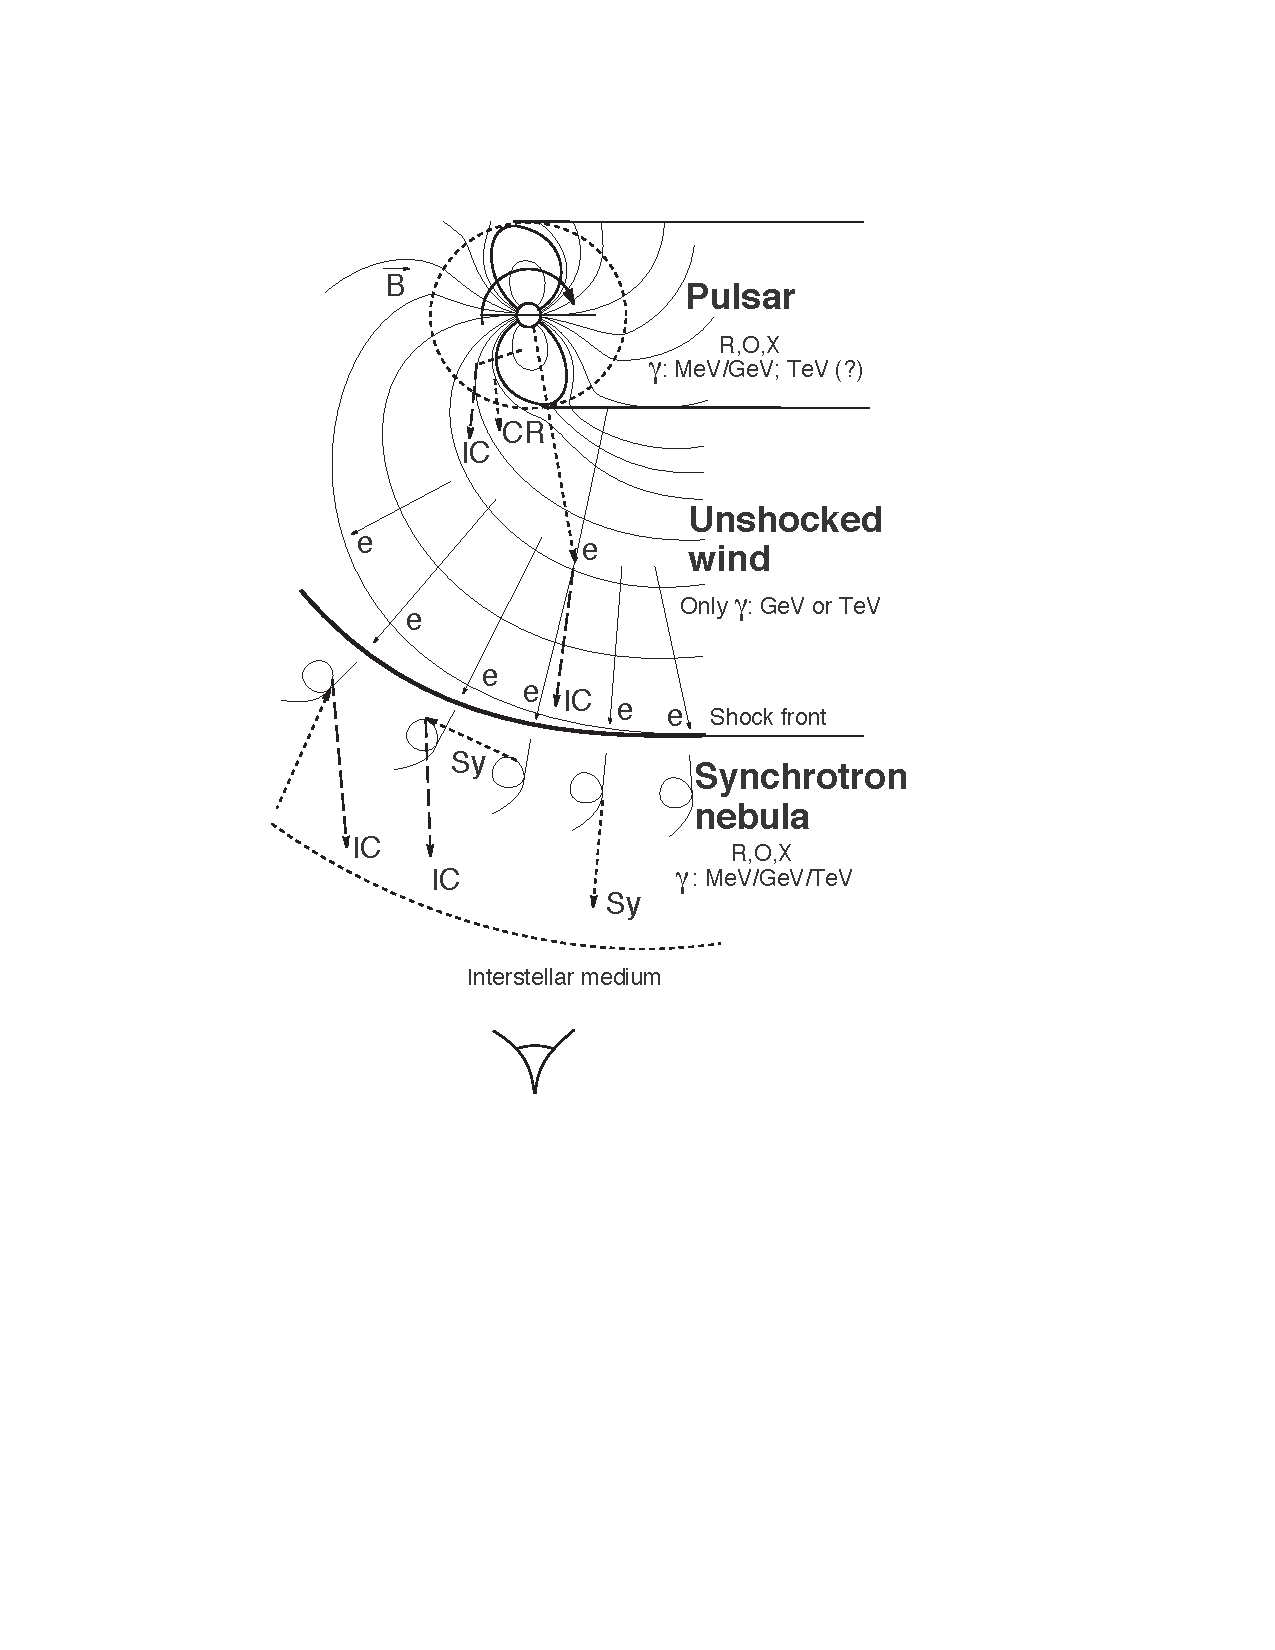
\includegraphics{chapters/pulsar_pwn_system/figures/termination_shock.pdf}
  \end{center}
  \caption{The regions of emission in a pulsar/\ac{PWN} system. 
  This figure shows (top) the pulsar's magnetopshere, (middle), the
  unshocked pulsar wind and (bottom) the shocked pulsar wind which can
  be observed as the \ac{PWN}.
  ``R'', ``O'', ``X'', and ``$\gamma$'' describe sites of radio, optical, X-ray, and
  $\gamma$-ray emission respectivly.
  ``CR'', ``Sy'', and ``IC'' refer to regions of curvature, inverse Compton, and
  synchrotron emission.
  Figure is taken from \cite{aharonian_2003_exploring-physics}.
  }
  \figlabel{termination_shock}
\end{figure}

The radius of the bubble (\radiusterminationshock) is the
radius where the ram pressure from the wind equals the pressure of the
gas in the \ac{SNR}. 
The ram pressure is computed as the energy in the
bubble $\energydot \radiusterminationshock/c$ (assuming the particles
travel with a velocity $\approx \speedoflight$) divided by the volume
$4\pi\radiusterminationshock^3/3$:
\begin{equation}
  \radiusterminationshock = \sqrt{\frac{\energydot}{\tfrac{4}{3}\pi \pressureISM \speedoflight}}.
\end{equation}
Here, \pressureISM is the pressure in the SNR.
Typical values for the termination shock are 0.1\unitspace\parsec
which is an angular size $\sim$ \ac{arcsec} for distances $\sim\kiloparsec$
\citep{gaensler_2006_evolution-structure}.

At the termination shock, the particles are
thermalized (given a random pitch angle), and accelerated
to energies of $10^{15}\unitspace\electronvolt$
\citep{arons_1996_pulsars-gamma-rays}.

Downstream of the shock, the particles emit synchotron and \ac{IC}
radiation as the thermalized electron population interacts with the
magnetic filed and seed photons \citep{gaensler_2006_evolution-structure}.

\figref{termination_shock} shows a
diagram describing magnetosphere, unshocked wind, and synchrotron
nebula which make up the Pulsar/\ac{PWN} system.



\begin{itemize}
  \item ``Following this discovery, a theoretical understanding was
  soon developed in which the central pulsar generates a magnetized
  particle wind, whose ultrarelativistic electrons and positrons radiate
  synchrotron emission across the electromagnetic spectrum (Pacini \&
  Salvati 1973, Rees \& Gunn 1974). The pulsar has steadily released
  about a third of its total reservoir of ???? ergs
  of rotational energy into its surrounding nebula over the last 950
  years. This is in sharp contrast to shell-like SNRs, in which the
  dominant energy source is the ??? ergs of kinetic energy
  released at the moment of the original SN explosion.''  -- \cite{gaensler_2006_evolution-structure}
  \item How is pulsar outflow accelerated at shock?
  \item Discuss magnetization stuff :
    \begin{enumerate}
      \item see page 76 in "Relativistic Astrophysics and Cosmology" by Shapiro
    \end{enumerate}
\end{itemize}

\todo[inline]{Discuss pulsar evolution ``The Evolution and Structure of
Pulsar Wind Nebulae'' -- Bryan M. Gaensler and Patrick O. Slane}

\todo[inline]{Describe Mattana's work on \glspl{PWN}: ``On the evolution of
the Gamma- and X-ray luminosities of Pulsar Wind Nebulae''}


"As has been discussed, pulsar wind nebulae are prominent sources of
very high energy γ-rays. At these wavelengths, emission is caused
by inverse Compton acceler- ation of seed photons by the relativistic
electrons present in the nebula (see Section 1.3.5). As the electron
energies needed to boost photons to these energies are not as large as
that required for synchrotron emission to occur, inverse Compton emission
is seen at the extremes of the nebula where synchrotron emission can no
longer be observed and as such older pulsar wind nebulae are observed to
be much larger in VHE γ-rays than their X-ray counterparts. In addition
to this, inverse Compton emission is seen in the unshocked wind area of
the PWN as the electrons present are energetic enough to produce inverse
Compton radiation even if they are unable to produce synchroton radiation"
-- keogh\_2010\_search-pulsar


"The morphology of a young PWN is often elongated along the pulsar spin
axis due to the higher equatorial pressure associated with the toroidal
magnetic field (Begelman \& Li 1992, van der Swaluw 2003). This effect
is seen clearly in many PWNe (e.g., Figs. 1 \& 5) and allows one to infer
the likely projected orientation of the pulsar. As the nebula expands (see
§3.1), Rayleigh-Taylor instabilities form as the fast-moving relativistic
fluid encounters and accelerates slower-moving unshocked supernova
ejecta. These form dense, finger-like fillamentary structures that suffer
photoionization from the surrounding synchrotron emission and radiate
recombination lines in the optical and ultraviolet (UV) bands (Fig. 1(b);
Hester et al. 1996). The increased density compresses the magnetic field
around the fillaments, causing enhanced synchrotron emission. One
thus observes radio structures that correspond to the optical/UV
fillaments." -- \url{http://arxiv.org/pdf/astro-ph/0601081v1.pdf}

\todo[inline]{Describe SNR Reverse Shock}

"In later stages the PWN interacts with the reverse shock formed in the
SNR in which the NS was born. This interac- tion causes the disruption of
the PWN, often leading to composite SNRs with complicated PWN structures
in their interiors." -- slane\_2005\_young-neutron

"The structure of a PWN can be altered significantly through interaction
with the reverse shock from the SNR in which it resides. In its early
evolution the PWN is basically freely-expanding, encountering only small
amounts of slow- moving ejecta in the SNR interior. As the SNR blast
wave sweeps up sufficient amounts of circumstellar/interstellar material,
a reverse shock is driven back through the ejecta. As this reverse shock
propagates, heating the ejecta, it will eventually reach the PWN."
-- slane\_2005\_young-neutron

